\section{Data and Software}

\subsection{Data}
In this experimental setup, I used minute-binned OHLC data of crypto/USD-pairs obtained from the cryptocurrency 
exchange \href{ https://www.bitfinex.com/ }{Bitfinex} ranging from 01.01.2019 to 31.12.2019 via its official API.
For each minute-bin, \textit{Open}, \textit{High}, \textit{Low}, \textit{Close}, \textit{Volume} 
and \textit{Timestamp} data got collected. 
\textit{High} and \textit{Low} denote the highest and lowest price respectively
that was traded within this timeframe. 
\textit{Open} and \textit{Close} denote the first and last traded price.
\textit{Volume} denotes the total volume traded within the respective minute-bin.
\textit{Timestamp} denotes the point in time for each minute-bin as a UNIX-Timestamp,
i.e., is the number of seconds that have passed since 01.01.1970.

Even though Bitfinex is the largest exchange for cryptocurrency 
with a daily trading volume of roughly 111 million USD and
155 different Dollar-tradable coins \cite{bitfinex2012},
for most coins, the trading frequency is so low such that 
many crypto/USD-pairs have a considerable amount of minute-bins in 
which no volume was traded (see figure \ref{fig:all_missing_bins_total}).

\begin{figure}[H] 
    \captionsetup{format=plain}
    \makebox[\textwidth]{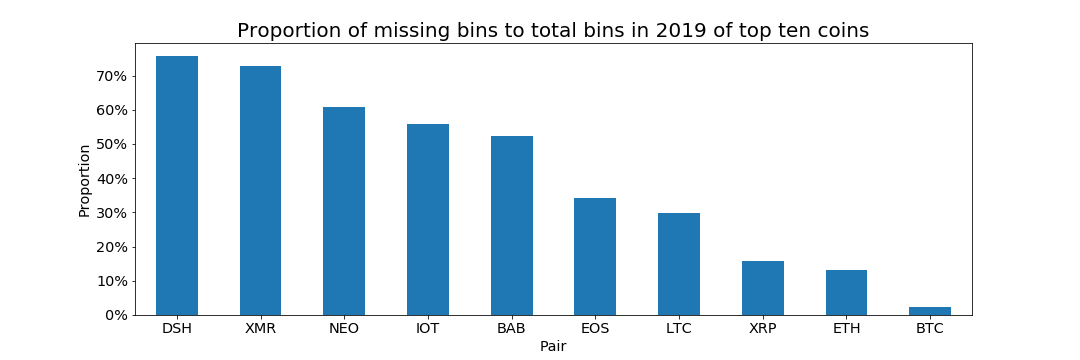
\includegraphics[width=200mm]{all/all_missing_bins_total.png}}
    \caption{
        This figure illustrates the proportion of missing minute-bins
        to total number of minute-bins in 2019 for the top ten coins.
    }
    \label{fig:all_missing_bins_total}
\end{figure}


In case of a crypto-pair having no volume for a particular minute, the API leaves out this bin
when requesting its data resulting in missing bins. 
This issue got resolved by propagating price values from the last active minute-bin
and setting the volume to zero. Further, I restricted the number of crypto/USD-pairs to the
top ten pairs by market capitalization \cite{coinmarketcap2013}. 
In addition, I decided to only take data from 01.01.2019 to 31.12.2019, 
since 2019 was the most active year in terms of trading frequency for most coins.
Thus, the resulting data set contains roughly
$ 10\, \times\, 365\, \times\, 24\, \times\, 60\, = 5.256.000 $ rows.



\subsection{Software}
The programming language used for conducting this study is Python 3.7 \cite{python2020}.
For data preparation and feature engineering, I used Pandas and numpy (\cite{pandas2020}, \cite{numpy2020}).
Data Visualization was done via Maplotllib \cite{matplotlib2020}.
I used the respective Scikit-learn implementation of the Machine Learning models used in this master thesis \cite{scikit2020}. 
